\documentclass[10pt,a4paper]{article}

% === PAQUETES === (((
\usepackage{amsmath}
\usepackage[shortlabels]{enumitem}
\usepackage{amsfonts}
\usepackage{ragged2e}
\usepackage{subfigure}
\usepackage{amssymb}
\usepackage{slashbox}
\usepackage{multirow}
\usepackage{multicol}
\usepackage{fontspec}
\usepackage{fullpage}
\usepackage{graphicx}
\usepackage{titlesec} 
% \usepackage{setspace}
\usepackage{dsfont}
% \usepackage{bookmark}
% )))

% === TIPOGRAFÍA === (((
\setmainfont[
  BoldFont       = bodonibi,
	ItalicFont     = Century modern italic2.ttf,
	BoldItalicFont = bodonibi,
	SmallCapsFont  = lmromancaps10-regular.otf
]{Century_modern.ttf}
% )))

% === COMANDOS === (((
\newcommand{\dis}{\displaystyle}
\newcommand{\qed}{\hspace{0.5cm}\rule{0.16cm}{0.4cm}}
\newcommand{\micita}[1]{\([\)\cite{#1}\(]\)}
\newcommand{\operator}[1]{\mathop{\vphantom{\sum}\mathchoice{ \vcenter{\hbox{\huge $#1$}} }
{\vcenter{ \hbox{\Large $#1$}} }{#1}{#1}}\displaylimits}
\newcommand{\suma}{\operator{ 
\includegraphics[scale=0.09]{IMAGENES/Sigma.png}} }
\DeclareSymbolFont{italics}{\encodingdefault}{\rmdefault}{m}{it}
\DeclareSymbolFontAlphabet{\mathit}{italics}
\ExplSyntaxOn
\int_step_inline:nnnn { `A } { 1 } { `Z }
 {  \exp_args:Nf \DeclareMathSymbol{\char_generate:nn{#1}{11}}{\mathalpha}{italics}{#1} }
\int_step_inline:nnnn { `a } { 1 } { `z } {  \exp_args:Nf \DeclareMathSymbol{\char_generate:nn{#1}{11}}{\mathalpha}{italics}{#1}}
\ExplSyntaxOff
% )))

% === SECCIONES === (((
\titleformat*{\section}{\large\normalfont\bfseries}
\titleformat*{\subsection}{\large\itshape \centering}
% \setcounter{secnumdepth}{0}
\renewcommand*{\contentsname}{\large\textbf{CONTENIDOS.}}
\usepackage[nottoc,numbib]{tocbibind}
\renewcommand{\refname}{REFERENCIAS.}
\renewcommand{\tablename}{Tabla}
\renewcommand{\figurename}{Figura}
% )))

% === PORTADA === (((
% \pagestyle{empty}
\newcommand{\portada}{
\addfontfeature{LetterSpace=-5}
  \begin{titlepage}
  \centering
  \begin{figure}
    \centering
    
\includegraphics[scale=0.5]{IMAGENES/logo_uaa.png}  
  \end{figure}
  {\bfseries\Large\MakeUppercase{\textit{Universidad Autónoma de Aguascalientes.}} \par}
  \vspace{1cm}
  {\Large Centro de Ciencias Básicas. \vspace{0.5cm}\\[2mm]
  Departamento de Matemáticas y Física.\vspace{0.5cm}\\[2mm]
  Licenciatura en Matemáticas Aplicadas.\vspace{0.5cm}\\[2mm]
  Práctica 6.\par}
  \vspace{1.5cm}
  {\bfseries\Huge Experimento de Young. \par} % title
  \vspace{1.5cm}
  {\itshape\Large Óptica. \\Prof. Mariana Alfaro Gómez.\par}
  % {\itshape\Large Variable Compleja I. \\Prof. Fausto Arturo Contreras Rosales.\par}
  % {\itshape\Large Métodos Numéricos II. \\Prof. Manuel Ramírez Aranda.\par}
  % {\itshape\Large Diseño de Experimentos. \\Prof. Angélica Hernández Quintero.\par}
  % {\itshape\Large Filosofía de la Investigación Científica. \\Prof. Jesús Mariano Rodríguez Muñoz.\par}
  \vfill
  % {\Large \textit{Por Erick I. Rodríguez Juárez.}\par}
		\begin{flushleft}
		\Large
		Alumnos:\\
		\textit{Carlos Francisco Guzmán Barba.}\\
		\textit{Erick Ignacio Rodríguez Juárez.}\\
		\textit{Manuel Alejandro Siller Landin.}
		\end{flushleft}
	% {}  % {\Large \textit{Por Erick I. Rodríguez Juárez.}\par}
  \vfill
		\begin{flushright}
		{\Large Realización: 2\(/\)05\(/\)22. \par} % date
		{\Large Entrega: 16\(/\)05\(/\)22. \par} % date
		\end{flushright}
  \end{titlepage} 
	% \thispagestyle{empty}
	% \doublespacing
	% \tableofcontents
	% \singlespacing
	% \newpage
} 
% )))

\begin{document}

\portada

\section{RESUMEN.} % (((
Para esta práctica se construyó, mediante dos lentes convergentes de distinta distancia focal, un artefacto denominado microscopio, el cual nos permite visualizar los objetos que se enfoquen con éste de manera amplificada, es decir, que la magnificación total del objeto (en valor absoluto) sea mayor a uno. Para ello se estimó, tanto de manera práctica como teórica, la magnificación de un objeto con este microscopio, obteniéndose que la diferencia entre el valor práctico y el valor teórico de dicha magnificación total era de $0.4453\pm 0.0464$, lo que confirma entonces que este instrumento óptico permite amplificar los objetos en la manera que sea necesaria, siempre y cuando se comprenda el funcionamiento de las lentes delgadas de modo que, combinándolas correctamente, se obtenga el aumento de la imagen deseado.
% )))

\section{INTRODUCCIÓN.} % (((

\subsection{--- Lentes Individuales ---} % (((
\label{sub:lentes_individuales}
Recordemos que la imagen producida por un objeto en una lente convergente queda completamente determinada por dos rayos.
El rayo que pasa por el centro de la lente (sin desviarse) y el que es paralelo al eje óptico y es colimado al pasar por el foco \(F_i\) del lado opuesto.
En la Figura \ref{fig:lente} (obtenida de \micita{alonso_finn}), se tiene el objeto ubicado entre el foco \(F_o\) y la lente, entonces la imagen producida será virtual y vertical.
\begin{figure}[ht]
	\centering
	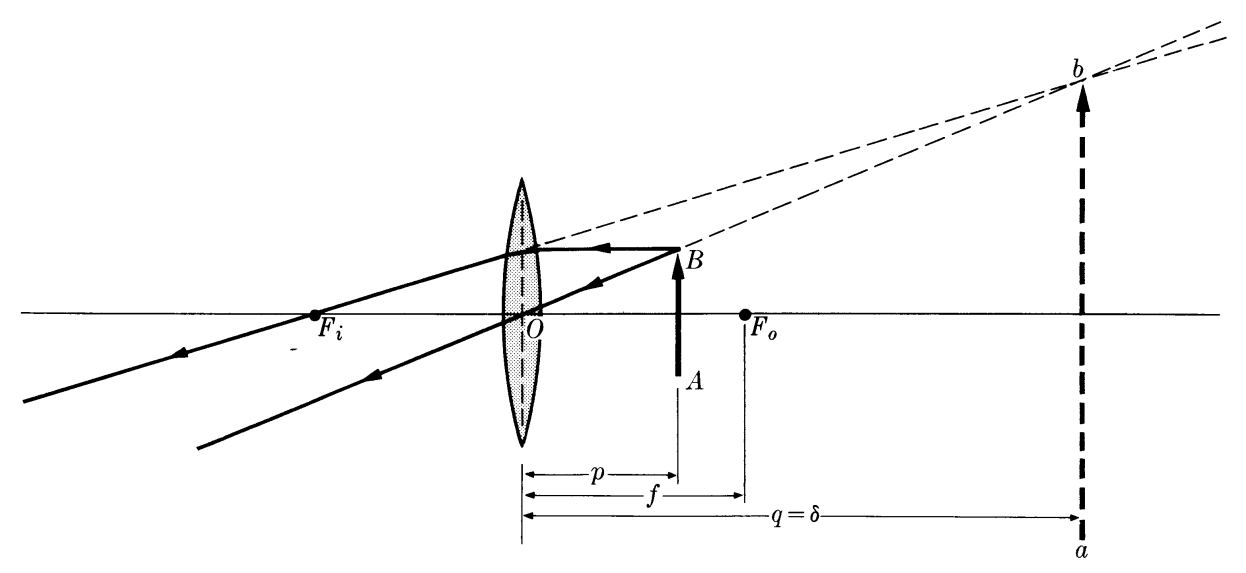
\includegraphics[width= 0.8 \linewidth]{IMAGENES/1_INTRO/lente_simple.png}
	\caption{Trazo de rayos de una lente convergente, el objeto entre el foco y la lente.}
	\label{fig:lente}
\end{figure}\\
Recordemos que, por la definición de \textit{magnificación}, obtenemos \(M = \dfrac{ab}{AB}\).
Notar que ambos triángulos comparten el mismo ángulo en el punto \(O\), entonces \(M=q/p\), y con la notación \(d_o=p\), \(-d_i=q\), obtenemos
\begin{equation}
	M = -\dfrac{d_i}{d_o}.
	\label{eq:magnificacion}
\end{equation}
Así, modificando la posición de la lente, se modificará la magnificación por (\ref{eq:magnificacion}).
Obsérvese que las distancias objeto e imagen satisfacen los siguiente.
\begin{equation}
	\dfrac{1}{d_o} + \dfrac{1}{d_i} = \dfrac{1}{f}.
	\label{eq:ley_lentes}
\end{equation}
Esto dice que, si \(d_o=f\), entonces \(d_i= \infty\). Y por tanto, \(M= \infty\).
Entonces la imagen (virtual) será mayor cuando el objeto se acerque al foco \(F_o\) de la lente, puesto que las líneas puntadas serán paralelas, cuando el segmento \(AB\) pase por \(F_o\).
% )))

\subsection{--- Microscopio Compuesto ---} % (((
\label{sub:microscopio_compuesto}
Un \textbf{microscopio compuesto} es un sistema de dos lentes (objetivo y ocular) que producen una imagen virtual aumentada e invertida de un objeto pequeño, así como lo indica la Figura \ref{fig:microscopio} (también obtenida de \micita{alonso_finn}).
\begin{figure}[ht]
	\centering
	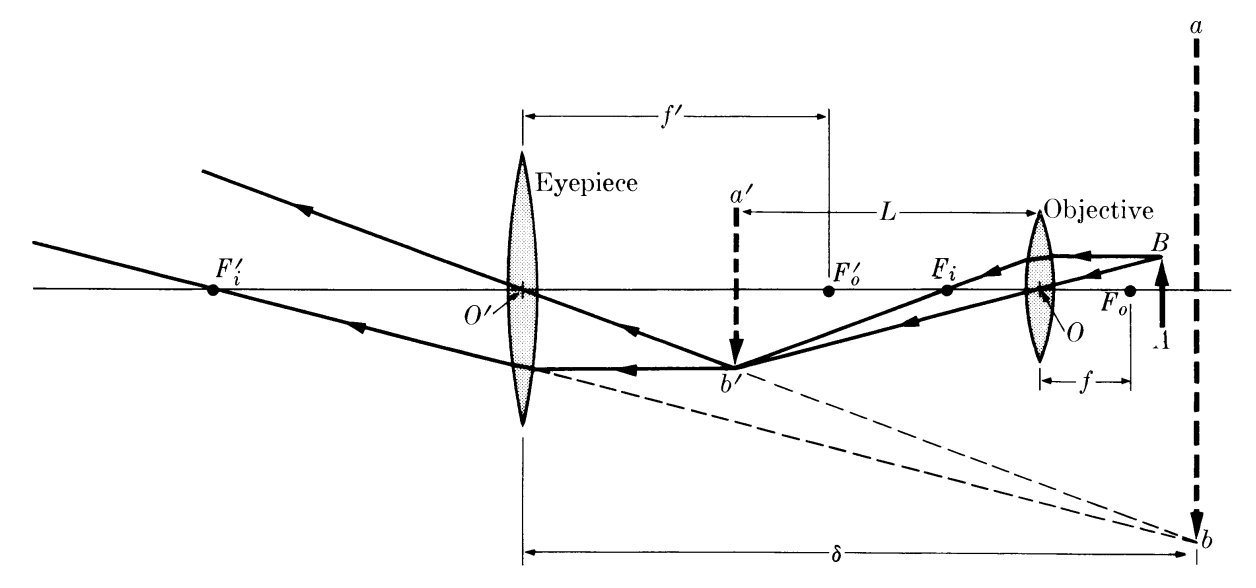
\includegraphics[width= 0.8 \linewidth]{IMAGENES/1_INTRO/microscopio.png}
	\caption{Sistema de lentes de un microscopio.}
	\label{fig:microscopio}
\end{figure}\\
La lente objetivo, al colocarse su foco \(F_o\) por delante del objeto \(AB\), produce una imagen invertida y real.
Mientras que la lente ocular, al tener la imagen \(a'b'\) producida por la lente objetivo, como objeto, se encuentra en la situación de la sección \ref{sub:lentes_individuales}, y tendrá un imagen virtual aumentada.
Así, la imagen final \(ab\) es aumentada, invertida, y virtual.\\

La magnificación de la lente objetivo es \(M_{objetivo} = a'b' /AB\).
La magnificación de la lente ocular es \(M_{ocular} = ab/a'b'\).
En términos de la notación utilizada en la práctica, se tiene \(M_{objetivo} = -d_{i1} /d_{o1}\), \(M_{ocular} = -d_{i2} / d_{o2}\).
Así, la magnificación total es:
\begin{equation}
	M = M_{objetivo} M_{ocular} = \left(-\dfrac{d_{i1}}{d_{o1}} \right)\cdot \left(-\dfrac{d_{i2}}{d_{o2}}\right).
	\label{eq:magnificacion_final}
\end{equation}
Se sabe que el sistema \(1/d_o+1/d_i=1/f\), \(d_i+d_o=k\), tiene sólo dos soluciones, que indican dónde se formará una imagen (final, invertida, ampificada) nítida, en el sistema de una sola lente.
Además, como se vio en la sección \ref{sub:lentes_individuales}, cuanto más se acerque la imagen de la lente objetivo, al foco de la lente ocular, es decir, cuando \(d_{o2} =f_2\), se tendrá amplificación máxima. El proceso de encontrar la mayor amplificación posible de esta manera, se le llama \textit{enfocar}. El objetivo es montar las lentes de un microscopio compuesto y calcular su amplificación.
% )))

\subsection{--- Paralaje ---} % (((
\label{sub:paralaje}
Dado que el cuerpo humano posee dos lentes convergentes (dos ojos), ocurre la siguiente situación geométrica con cada uno de los objetos observados, como lo indica la Figura \ref{fig:paralaje}.
\begin{figure}[ht]
	\centering
	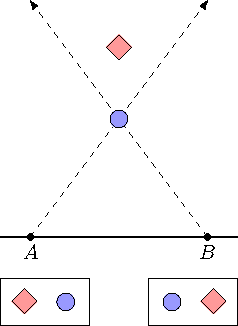
\includegraphics[width= 0.25 \linewidth]{IMAGENES/1_INTRO/1/tikz.pdf}
	\caption{Reflexión de las imágenes en cada uno de los observadores de la imagen.}
	\label{fig:paralaje}
\end{figure}
Esto dice, que no pueden observarse dos objetos al mismo tiempo con dos lentes diferentes preservando el mismo sentido.
% )))

% )))

\section{METODOLOGÍA.} % (((
\begin{enumerate}
	\item Se utilizaron 2 lentes convergentes convexas con una distancia focal de $100mm$ y $200mm$ como lente objetivo y lente ocular respectivamente.
	\item La mínima escala de la cinta métrica es $\dfrac{0.1cm}{2}=0.05cm$.
\end{enumerate}
La Figura \ref{fig:primer_fig} muestra la configuración para el dispositivo experimental usado. Se posiciona de manera paralela la pantalla, la lente objetivo y la lente ocular en ese orden mediante la ayuda de un banco óptico. \\[2mm]
\begin{figure}[ht]
	\centering
	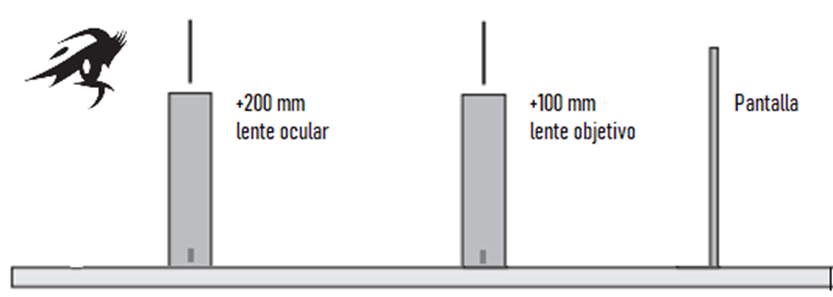
\includegraphics[width= 0.8 \linewidth]{METODOLOGIA/5}
	\caption{Configuración inicial del dispositivo experimental.}
	\label{fig:primer_fig}
\end{figure}\\
Dado que se requiere construir un microscopio y determinar su magnificación, es necesario poder tener una imagen nítida y referencial para poder medir, para ello, se procedió a poner una hoja cuadriculada en la pantalla como se muestra en la Figura \ref{fig:segunda_fig}. \\[2mm]
\begin{figure}[ht]
	\centering
	\includegraphics[width= 0.5 \linewidth, angle = -90,origin=c]{METODOLOGIA/1_nueva}
	\caption{Cuadrícula pegada en la pantalla.}
	\label{fig:segunda_fig}
\end{figure}\\
Ahora, moviendo solo la lente objetivo, se logró tener la posición en la que se tuvo una imagen nítida. A continuación, fue necesario mover la lente ocular de tal manera que se pudiese tener una referencia en el aumento sin paralaje, esto es, para alinear se tuvo que trabajar con ambos ojos, uno visualizando la hoja cuadriculada sin el uso de las lentes y el otro visualizando la hoja cuadriculada a través de las lentes, respectivamente el ojo izquierdo y derecho, para poder tener un aproximado en la potencia del microscopio como se muestra en la Figura \ref{fig:tercer_fig}, \ref{fig:cuarta_fig} y \ref{fig:quinta_fig}. \\[2mm]
\begin{figure}[ht]
	\centering
	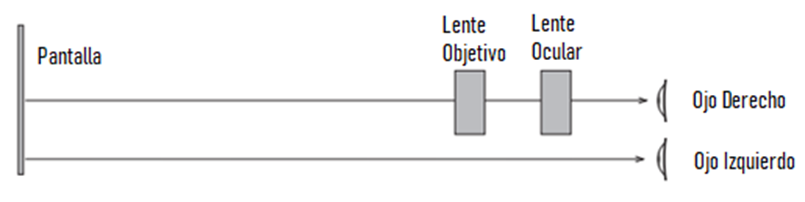
\includegraphics[width= 0.8 \linewidth]{METODOLOGIA/4}
	\caption{Visualización de objeto e imagen simultáneamente para eliminar paralaje.}
	\label{fig:tercer_fig}
\end{figure}\\
\begin{figure}[ht]
\begin{minipage}{0.5\linewidth}
	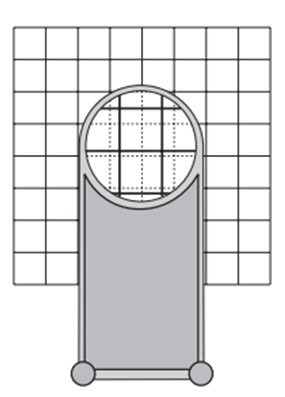
\includegraphics[width= 0.9 \linewidth]{METODOLOGIA/3}
	\caption{Observación del fenómeno de amplificación del objeto a través de las lentes.}
	\label{fig:cuarta_fig}
\end{minipage}\hspace{5mm}
\begin{minipage}{0.5\linewidth}
	\includegraphics[width= 0.9 \linewidth, angle = -90, origin = c]{METODOLOGIA/2_nueva}
	\caption{Vista de la Figura \ref{fig:tercer_fig} con la\\configuración del dispositivo experimental.}
	\label{fig:quinta_fig}
\end{minipage}
\end{figure}
Al tener todo posicionado de tal manera que se tenga una imagen nítida y referencial a la magnificación de la lente se procedió a registrar las posiciones sobre el banco óptico a la que se encontraba la pantalla y las lentes además de la magnificación observada del microscopio.
% )))

\newpage

\section{RESULTADOS.} % (((
Los resultados obtenidos al realizar el experimento fueron los siguientes (ver Tabla \ref{tab:resultados}). El cálculo de éstos valores se encuentra en la sección \ref{sec:apendice}.
\begin{table}[ht]
\centering
\caption{Resultados obtenidos de las mediciones.}
\begin{tabular}{|c|c|}
	\hline
	Posición de la lente objetivo & $ (43.15\pm0.05)cm $ \\ 	\hline
	Posición de la lente ocular & $ (14.85\pm0.05)cm $  \\ 	\hline
	Posición de la pantalla & $ (70\pm0.05) cm $  \\ 	\hline
	Magnificación observada & $ 2 $ \\ 	\hline
	$d_{o1}$ & $ (26.85\pm 0.05) cm $  \\ 	\hline
	$d_{i2}$ & $ (-32.3916\pm 0.2871) cm $ \\ 	\hline
	$d_{i1} $ & $ (15.9347\pm0.0769)cm $  \\ 	\hline
	$d_{o2}$ & $ (12.3652\pm0.1769)cm $  \\ 	\hline
	Magnificación calculada & $ -1.5546\pm0.0464 $  \\ 	\hline
	Error absoluto &  $ |2-1.5546|=0.4453 $\\ 	\hline
\end{tabular}
	\label{tab:resultados}
\end{table}\\
El trazo de rayos con los datos obtenidos queda en la Figura \ref{fig:rayos}.
\begin{figure}[ht]
	\centering
	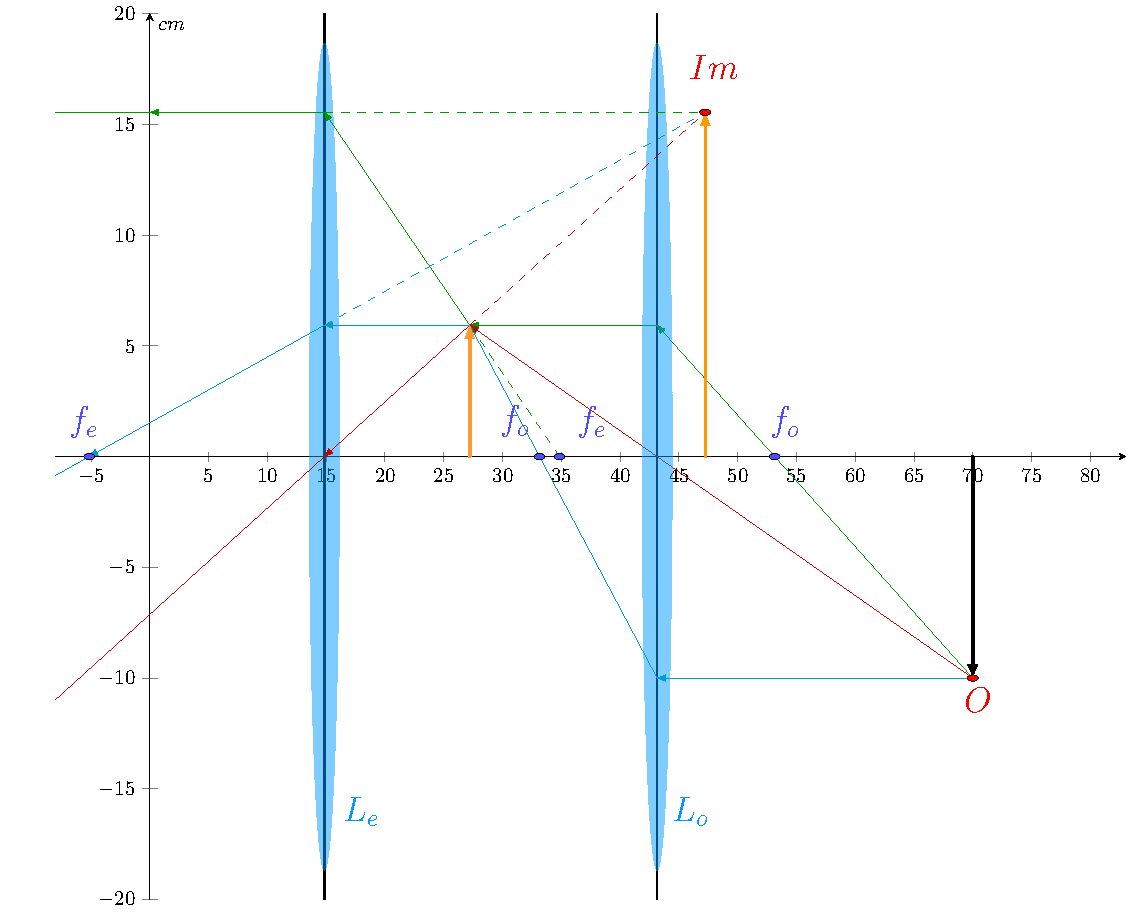
\includegraphics[height=11.5cm]{RESULTADOS/rayos.pdf}
	\caption{Trazado de rayos para el microscopio con las condiciones del laboratorio.}
	\label{fig:rayos}
\end{figure}
% )))

\newpage

\section{DISCUSIÓN DE RESULTADOS Y CONCLUSIONES.} % (((
En el desarrollo del experimento al momento de tener el ajuste de las lentes para tener la imagen nítida con el mínimo de paralaje, pudimos estimar el valor de la magnificación de $2$, lo que significa que al estar viendo mediante el ojo derecho la cuadrícula a través de las lentes, y con el ojo izquierdo la cuadrícula original, se pudo observar que visto desde el microscopio, un cuadrado de la cuadrícula contiene a $2$ cuadros de la cuadrícula observada para el objeto óptico. \\[2mm]

En la parte analítica se obtuvo un valor de magnificación para el microscopio de $-1.5546 \pm 0.0464$ con lo cual observamos que, en primera instancia, los valores entre lo observado y lo estimado indican que la imagen se encuentra derecha o invertida respectivamente.
Por otro lado, al analizar la teoría de lentes delgadas, vemos que ambas lentes del experimento, siendo convexas y convergentes, provocan una imagen final que es invertida respecto al objeto.
Adentro de la cuadrícula no hay un sentido de imagen derecha o imagen invertida por lo que fue natural dar la magnificación como un valor positivo; para corregir esto se pudo haber marcado la cuadrícula, de tal forma que las líneas verticales se les designara un sentido al marcarlas con flechas (ejemplo, un campo vectorial) para evitar problemas con el paralaje y la orientación, de esta manera se hubiese podido ver claramente a través de las lentes una imagen invertida con respecto al objeto pantalla reafirmando directamente lo analizado en la teoría para lentes delgadas. \\[2mm]

Es necesario hacer la observación de que la calidad de las lentes no era la mejor ya que para la Figura 4, la cual constituye al trazado de rayos del modelo experimental, no coincide la imagen con el objeto pantalla.
La teoría no falla, pero dada nuestra poca experiencia para decidir el enfoque de las lentes, implicó tener un margen de error de tal manera que la distancia final entre la imagen y la pantalla fue de $(22.7584\pm0.3371)cm$.
Lo ideal hubiese sido haber elaborado el trazado de rayos para verificar si la imagen deseada estuviese efectivamente posicionada en la pantalla, por lo que también es de esperarse que el valor estimado visualmente de la magnificación no fue obtenido de buena manera por lo argumentado anteriormente con respecto a la posición de la imagen y la pantalla.

Sin embargo, al final fue posible analizar el funcionamiento del microscopio tanto de manera práctica así como de manera teórica, y por ambos caminos se pudo estimar la magnificación en la imagen de este instrumento óptico, comparar tales valores, y comprobar que, efectivamente, el microscopio es útil para visualizar de manera amplificada los objetos. 
% )))

% === REFERENCIAS === (((
\bibliography{Referencias}
\bibliographystyle{unsrt}
% )))

\section{APÉNDICE.} % (((
\label{sec:apendice}
De la fórmula de lentes delgadas se sabe que 
$$\dfrac{1}{d_o}+\dfrac{1}{d_i}=\dfrac{1}{f}$$
Despejando $ d_i $ se tiene: \hspace{0.4cm} $d_i=\dfrac{d_o\cdot f}{d_o-f}$
Por otro lado, la incertidumbre para la suma, el producto y un cociente están dadas (respectivamente) por
\begin{align*}
	(x\pm \delta x)\pm(y\pm \delta y)&=(x\pm y)\pm(\delta x+\delta y)\\\\
	(x\pm\delta x)(y\pm\delta y)&=x\cdot y\pm\left(|y|\delta x+|x|\delta y \right)\\\\
	\dfrac{x\pm\delta x}{y\pm\delta y}&=\dfrac{x}{y}\pm\left(\dfrac{\delta x}{|y|}+|x|\dfrac{\delta y}{|y|^2}\right)
\end{align*}
Haciendo los cálculos para $ d_{i1} $
\begin{align*}
	d_{o1}\cdot f_1&=[(26.85\pm 0.05)cm](10cm)=\\	&=[(26.85\cdot10)\pm(0.05\cdot20)]cm^2=\\
	&=(268.5\pm0.5)cm^2\\\\
	d_{o1}-f_1&=[(26.85\pm 0.05)cm]-(10cm)=\\
	&=(16.85\pm0.05) cm
\end{align*}
Entonces
\begin{align*}
	d_{i1}&=\dfrac{d_{o1}\cdot f_1}{d_{o1}-f_1}=\\\\
	&=\dfrac{(268.5\pm0.5)cm^2}{(16.85\pm0.05) cm}=\\\\
	&=\left[\dfrac{268.5}{16.85}\pm\left(\dfrac{0.5}{16.85}+
	268.5\cdot\dfrac{0.05}{16.85^2}\right)\right]cm=\\\\
	&=(15.9347\pm0.0769)cm
\end{align*}
Ahora, para la distancia objeto con respecto a la lente ocular ($ L_e $), se tiene que
\begin{align*}
	d_{o2}&=(d_{L_o}-d_{i1})-d_{L_e}=\\
	&=[(43.15\pm0.05)cm-(15.9347\pm0.0769)cm]-(14.85\pm0.05)cm=\\
	&=(27.2152\pm0.1269)cm-(14.85\pm0.05)cm=\\
	&=(12.3652\pm0.1769)cm
\end{align*} 
Entonces, ahora haciendo los cálculos para obtener $d_{i2}$
\begin{align*}
	d_{o2}\cdot f_2&=[(12.3652\pm0.1769)cm](20cm)=\\
	&=\left[(12.3652\cdot20)\pm\left(0.1769\cdot20\right)\right]cm^2=\\
	&=(247.304\pm3.538)cm^2\\\\
	d_{o2}-f_2&=(12.3652\pm0.1769)cm-(20cm)=\\
	&=(-7.6348\pm0.1769)cm
\end{align*}
Así pues 
\begin{align*}
	d_{i2}&=\dfrac{d_o2\cdot f_2}{d_o2-f_2}=\dfrac{(247.304\pm3.538)cm^2}{(-7.6348\pm0.1769)cm}=\\\\
	&=\left[\dfrac{247.304}{-7.6348}\pm\left(\dfrac{3.538}{7.6348}+247.304\cdot\dfrac{0.1769}{7.6348^2}\right)\right]cm=\\\\
	&=(-32.3916\pm 0.2871)cm
\end{align*}
Los cálculos correspondientes para $M1$ son los siguientes
\begin{align*}
	M1&=-\dfrac{d_{i1}}{d_{o1}}=-\dfrac{(15.9347\pm0.0769)cm}{(26.85\pm 0.05) cm}=\\\\
	&=-\dfrac{15.9347}{26.85}\pm\left(\dfrac{0.0769}{26.85}+15.9347\cdot\dfrac{0.05}{26.85^2}\right)=\\\\
	&=-0.5934\pm0.0039 
\end{align*}
Y para $M2$
\begin{align*}
	M2&=-\dfrac{d_{i2}}{d_{o2}}=-\dfrac{(-32.3916\pm 0.2871) cm}{(12.3652\pm0.1769)cm}=\\\\
	&=-\dfrac{(-32.3916)}{12.3652}\pm\left(\dfrac{0.2871}{12.3652}+32.3916\cdot\dfrac{0.1769}{12.3652^2}\right)=\\\\
	&=2.6195\pm0.0606
\end{align*}
Con esto, se puede calcular la magnificación total
\begin{align*}
	M_T=M_1\cdot M_2&=(-0.5934\pm0.0039)(2.6195\pm0.0606)=\\\\
	&=(-0.5934)(2.6195)\pm\left(0.5934\cdot0.0606+2.6195\cdot0.0039\right)=\\\\
	&=-1.5546\pm0.0464 
\end{align*}
% )))

\end{document}
